\documentclass[10pt,a4paper]{article}
\usepackage[T1]{fontenc}
\usepackage[utf8]{inputenc}
\usepackage{enumitem}
\usepackage{graphicx}
\usepackage{tabularx}
\usepackage{multirow}
\usepackage{helvet}
\usepackage{verbatim}
\usepackage[hidelinks]{hyperref}
\usepackage[a4paper,margin=1in]{geometry}
\usepackage{float}
\usepackage[polish]{babel}

\renewcommand\familydefault{\sfdefault}

\begin{document}
\begin{titlepage}
	\centering
	{\Large Wydział Matematyki i Nauk Informacyjnych Politechniki Warszawskiej \par}
	\vspace{1cm}
	
\includegraphics[width=0.2\textwidth]{logo.png} \par
	\vspace{5cm}
	{\LARGE System informacji oraz sprzedaży biletów\\komunikacji miejskiej i międzymiastowej \par}
	\vspace{0.5cm}
	{\Large Bartłomiej Dach, Tymon Felski \par}
	\vspace{1.5cm}
	{\Large Wersja 1.0 \par}
	\vspace{1.5cm}
	{\Large \today \par}
\end{titlepage}
Lista zmian w dokumencie:
\begin{table}[H]
\def\arraystretch{1.5}
\begin{tabularx}{\textwidth}{|l|l|X|l|}
	\hline
	\textbf{Data} & \textbf{Autor} & \textbf{Opis zmian} & \textbf{Wersja} \\
	\hline
	16.10.2016 & Bartłomiej Dach, Tymon Felski & Określenie wymagań projektu oraz harmonogramu prac & 1.0 \\
	\hline
	17.10.2016 & Bartłomiej Dach, Tymon Felski & Specyfikacja architektury systemu & 1.1 \\
	\hline
	18.10.2016 & Bartłomiej Dach, Tymon Felski & Dodanie administratora & 1.2 \\
	\hline
	10.11.2016 & Tymon Felski & Dodanie wymagań systemowych, instrukcji uruchomienia i utrzymania & 1.3 \\
	\hline
	11.11.2016 & Tymon Felski & Dodanie opisu modelu danych, scenariuszy i raportu z testów akceptacyjnych & 1.4 \\
	\hline
\end{tabularx}
\end{table}

\tableofcontents
\newpage

\section{Specyfikacja}

\subsection{Opis biznesowy}
Niniejszy system służy do przechowywania danych o przewoźnikach i połączeniach komunikacji miejskiej oraz międzymiastowej. Składowane dane wykorzystywane są do wyszukiwania konkretnych połączeń oraz sprzedaży biletów.

\subsection{Wymagania funkcjonalne}

\subsubsection*{Przypadki użycia}
Poniższy diagram UML przedstawia zbiór przypadków użycia aplikacji dla aktora -- pracownika firmy pośredniczącej w sprzedaży biletów wielu przewoźników.
\begin{figure}[H]
	\centering
	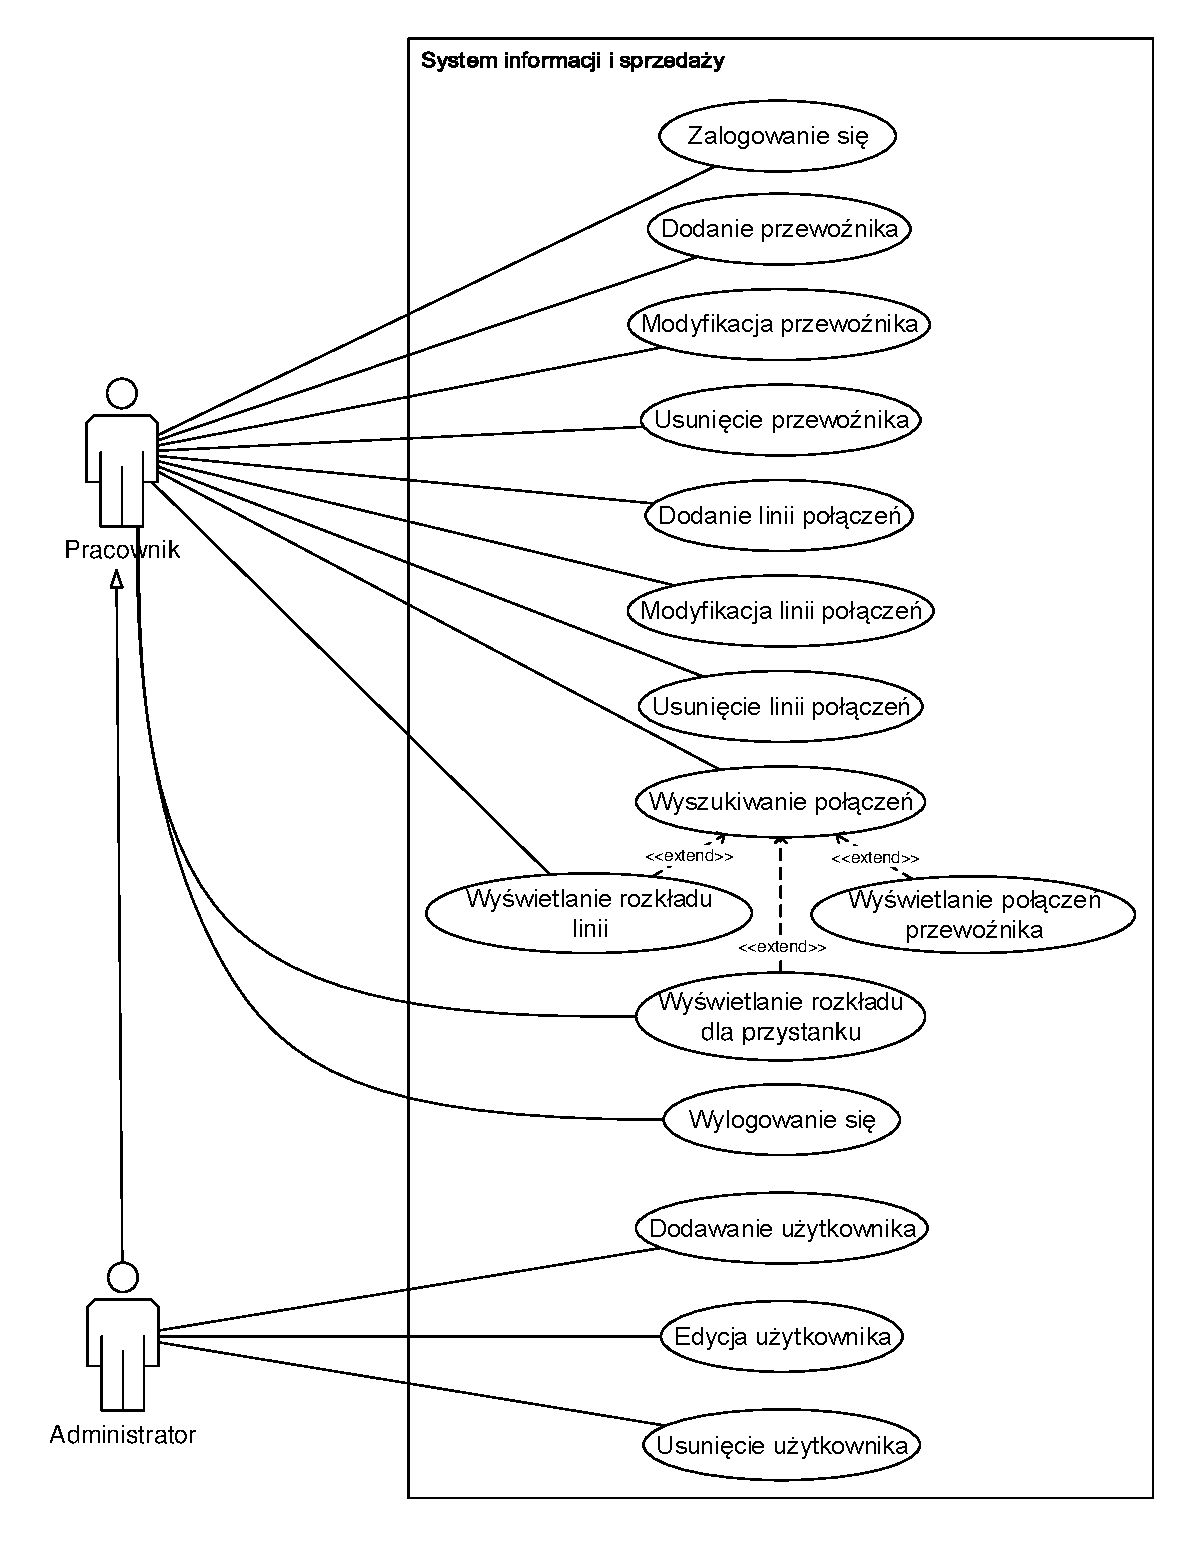
\includegraphics[width=12cm]{use-case.pdf}
	\caption{Diagram przypadków użycia dla aplikacji}
\end{figure}
Poszczególne przypadki są opisane szerzej w poniższej tabeli:
\begin{table}[H]
	\begin{tabularx}{\textwidth}{|c|X|X|X|}
		\hline
		\textbf{Aktor} & \textbf{Nazwa} & \textbf{Opis} & \textbf{Odpowiedź systemu} \\
		\hline
		\multirow{6}{*}{\rotatebox[origin=c]{90}{Administrator}}
		& Dodanie użytkownika
		& Dodanie nowego użytkownika do systemu
		& Potwierdzenie dodania użytkownika \\
		\cline {2-4}
		& Modyfikacja użytkownika
		& Zmiana danych istniejącego użytkownika systemu
		& Potwierdzenie zmodyfikowania rekordu \\
		\cline{2-4}
		& Usunięcie użytkownika
		& Usunięcie konta użytkownika i jego danych z systemu
		& Potwierdzenie usunięcia użytkownika \\
		\hline
		\multirow{26}{*}{\rotatebox[origin=c]{90}{Pracownik}}
		& Zalogowanie się 
		& Zalogowanie się użytkownika do systemu
		& Potwierdzenie zalogowania się lub komunikat o błędzie \\
		\cline{2-4}
		& Dodanie przewoźnika
		& Dodanie informacji o nowym przewoźniku do bazy
		& Potwierdzenie dodania danych do bazy \\
		\cline{2-4}
		& Modyfikacja przewoźnika
		& Zmiana danych przewoźnika przechowywanych w bazie
		& Potwierdzenie zmodyfikowania rekordu \\
		\cline{2-4}
		& Usunięcie przewoźnika
		& Usunięcie danych przewoźnika przechowywanych w bazie
		& Potwierdzenie usunięcia rekordu \\
		\cline{2-4}
		& Dodanie linii połączeń
		& Dodanie nowej linii połączeń danego przewoźnika
		& Potwierdzenie dodania linii do bazy \\
		\cline{2-4}
		& Modyfikacja linii połączeń
		& Modyfikacja linii połączeń danego przewoźnika
		& Potwierdzenie modyfikacji rekordu \\
		\cline{2-4}
		& Usunięcie linii połączeń
		& Usunięcie linii połączeń danego przewoźnika
		& Potwierdzenie usunięcia rekordu \\
		\cline{2-4}
		& Wyświetlanie rozkładu
		& Wyświetlanie rozkładu jazdy wybranej linii
		& Widok zawierający informacje o przejazdach na wybranej linii \\
		\cline{2-4}
		& Wyświetlanie połączeń przewoźnika
		& Wyświetlanie połączeń obsługiwanych przez danego przewoźnika
		& Widok zawierający informacje o liniach danej firmy \\
		\cline{2-4}
		& Wylogowanie się
		& Wylogowanie się pracownika z systemu
		& Potwierdzenie zakończenia pracy z systemem \\
		\hline
	\end{tabularx}
	\caption{Opisy przypadków użycia dla użytkownika}
\end{table}

\subsubsection*{User stories}
\begin{enumerate}
	\bfseries
	\item Interfejs administracyjny dla administratora
	\begin{enumerate}[label*=\arabic*.]
		\mdseries
		\item Jako zalogowany administrator dodaję/modyfikuję użytkownika systemu.\\
			Dowolny zalogowany administrator może dodać nowego użytkowanika lub zmodyfikować informacje o istniejącym użytkowniku, takie jak jego login, hasło oraz uprawnienia.
		\item Jako zalogowany administrator wyszukuję użytkownika. \\
		    Dowolny zalogowany administrator może wyszukać istniejących użytkowników systemu.
	\end{enumerate}
	\item Interfejs administracyjny dla pracownika
	\begin{enumerate}[label*=\arabic*.]
		\mdseries
		\item Jako zalogowany pracownik dodaję/modyfikuję przewoźnika. \\
			Dowolny zalogowany pracownik może dodać nowego przewoźnika lub zmodyfikować informacje o przewoźniku, takie, jak: nazwę i adres firmy, numer REGON oraz jej stronę internetową.
		\item Jako zalogowany pracownik dodaję/modyfikuję linię połączeń. \\
			Dowolny zalogowany pracownik może dodać nowe połączenie lub zmodyfikować informacje o istniejącym połączeniu takie jak: przystanki , czas odjazdu i przyjazdu na poszczególnych przystankach, ilość dostępnych miejsc w danym kursie, podstawowa cena biletu.
		\item Jako zalogowany pracownik wyszukuję połączenie. \\
		    Dowolny zalogowany pracownik może wyszukać dostępne połączenia pomiędzy
		    wprowadzonymi miastami.
	 	\item Jako zalogowany pracownik wyświetlam rozkład jazdy danej linii. \\
		    Dowolny zalogowany pracownik może wyszukać rozkład jazdy dla danej linii
		    komunikacyjnej i go wyświetlić.
    	\item Jako zalogowany pracownik wyświetlam połączenia dla danego przewoźnika. \\
		    Dowolny zalogowany pracownik może wyświetlić połączenia od danego przewoźnika.
	\end{enumerate}
\end{enumerate}

\subsection{Wymagania niefunkcjonalne}
Poniższa tabela zawiera rozpisane wymagania niefunkcjonalne narzucone dla systemu.
\begin{table}[H]
	\begin{tabularx}{\textwidth}{|c|l|X|}
		\hline
		\textbf{Obszar wymagań} & \textbf{Nr} & \textbf{Opis} \\
		\hline
		\multirow{5}{*}{Użyteczność (\textit{Usability})}
		& 1 & Rozmiar czcionki użytej w aplikacji musi być nie mniejszy niż 12 punktów. \\
		\cline{2-3}
		& 2 & Aplikacja powinna obsługiwać zmianę rozmiaru okna w sposób który umożliwia korzystanie ze wszystkich jej funkcjonalności (tzw. responsive design). \\
		\hline
		\multirow{3}{*}{Niezawodność (\textit{Reliability})}
		& 3 & Aplikacja musi być odporna na dokonywanie jednoczesnych zmian tego samego rekordu bazy przez wielu pracowników jednocześnie. \\
		\hline
		\multirow{7}{*}{Wydajność (\textit{Performance})}
		& 4 & Aplikacja powinna dodawać nowe obiekty do systemu w czasie nie dłuższym niż 1 sekundę, przy 50 żądaniach dodania obiektu na minutę. \\
		\cline{2-3}
		& 5 & Zużycie pamięci RAM przez aplikację nie powinno przekroczyć 200 megabajtów. \\
		\cline{2-3}
		& 6 & Wyszukiwanie połączenia między określonymi miastami powinno trwać mniej niż 2 sekundy, przy ok. 10 tys. rekordów. \\
		\hline
		\multirow{2}{*}{Utrzymanie (\textit{Supportability})}
		& 7 & Do aplikacji dołączona zostanie instrukcja wykonywania kopii zapasowej danych. \\
		\hline
	\end{tabularx}
	\caption{Tabela wymagań niefunkcjonalnych}
\end{table}

\subsection{Harmonogram projektu}
Prace przy projekcie będą realizowane według następującego harmonogramu:
\begin{figure}[H]
	\centering
	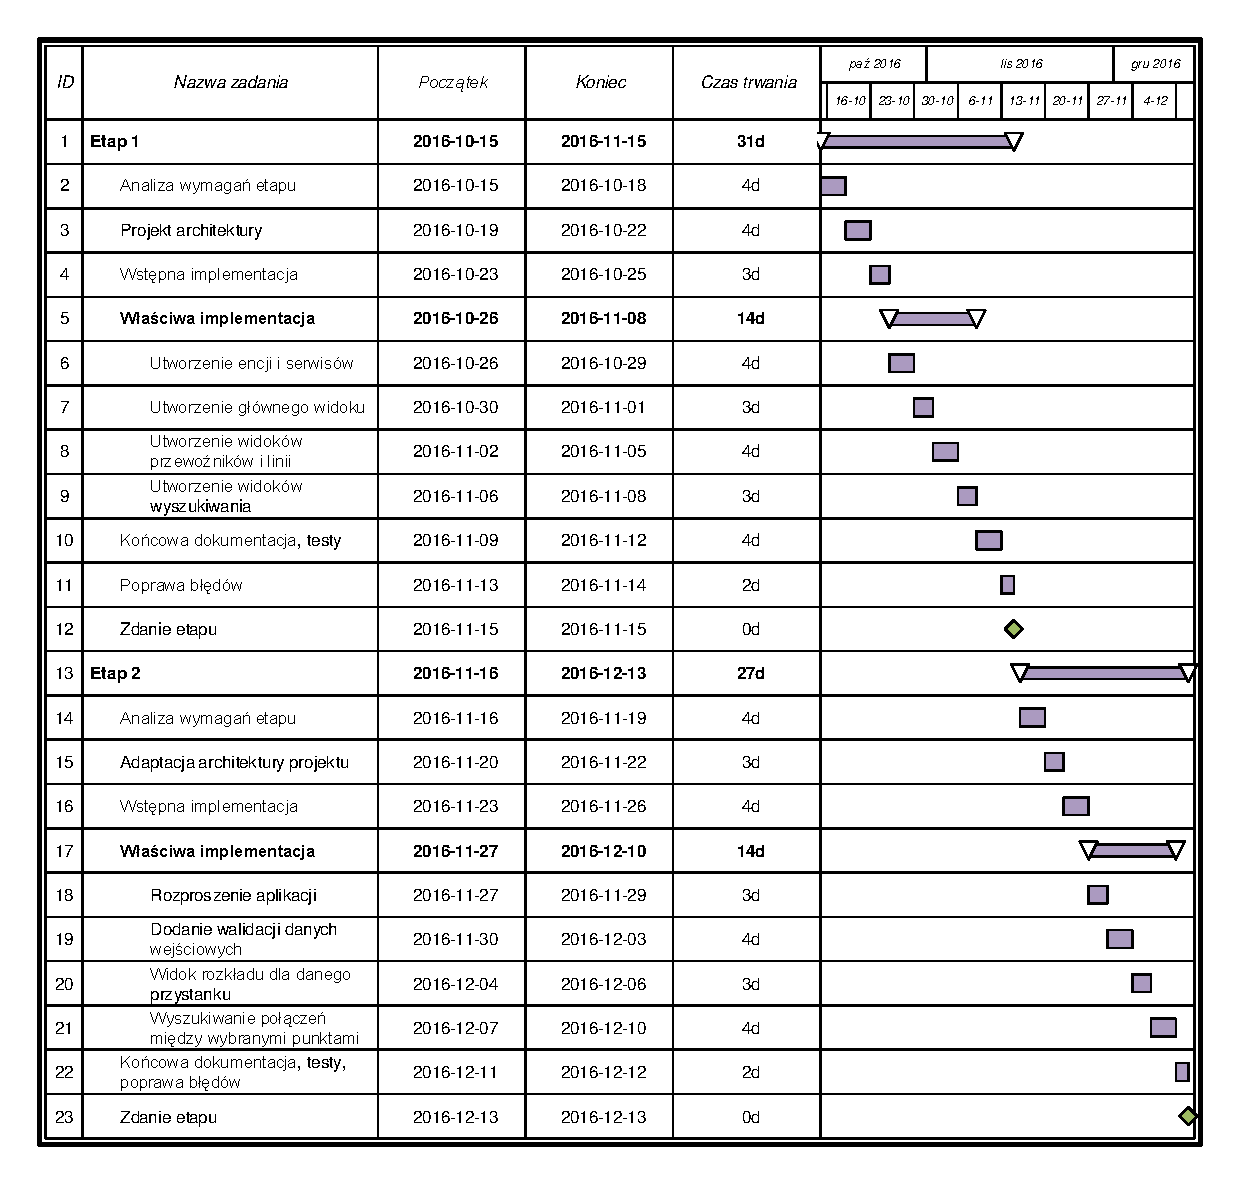
\includegraphics[width=16cm]{gantt.pdf}
	\caption{Diagram Gantta z planowanym harmonogramem projektu}
\end{figure}
Kamienie milowe:
\begin{enumerate}
	\item 18 października: Zakończenie analizy wymagań funkcjonalnych i niefunkcjonalnych projektu.
	\item 22 października: Zakończenie projektu architektury aplikacji, łącznie z wyróżnieniem komponentów oraz podsystemów.
	\item 25 października: Wstępna implementacja projektu architektury, naniesienie ewentualnych poprawek do architektury wynikających z problemów implementacyjnych.
	\item 29 października: Utworzenie encji biznesowych oraz serwisów wykorzystywanych przez użytkowników.
	\item 1 listopada: Utworzenie głównego widoku aplikacji.
	\item 5 listopada: Utworzenie widoków dodawania przewoźników oraz linii.
	\item 8 listopada: Utworzenie widoków wyszukiwania połączeń oraz wyświetlania połączeń danej linii oraz przewoźnika.
	\item 12 listopada: Zakończenie dokumentacji, testów aplikacji oraz identyfikacji błędów.
	\item 15 listopada: Zakończenie poprawy znalezionych błędów, zdanie projektu łącznie z pełną dokumentacją.
\end{enumerate}

\subsection{Architektura rozwiązania}
Docelowym środowiskiem aplikacji są małe lub średnie firmy pośredniczące w sprzedaży biletów komunikacyjnych, tzn. przedsiębiorstwa zatrudniające do 250 pracowników, z czego dostęp do systemu miałby dość niski procent tej liczby (w założeniach ok. 20-30\%). Dane, których przechowywanie jest niezbędne do spełnienia wymagań funkcjonalnych mają dość małą zmienność - stosunkowo rzadko ulegają zmianom lub przedawnieniom. Dodatkowo, ze względu na wewnętrzny charakter przechowywanych danych, system powinien być scentralizowany i znajdować się w jednym fizycznym położeniu.
\begin{figure}[H]
	\centering
	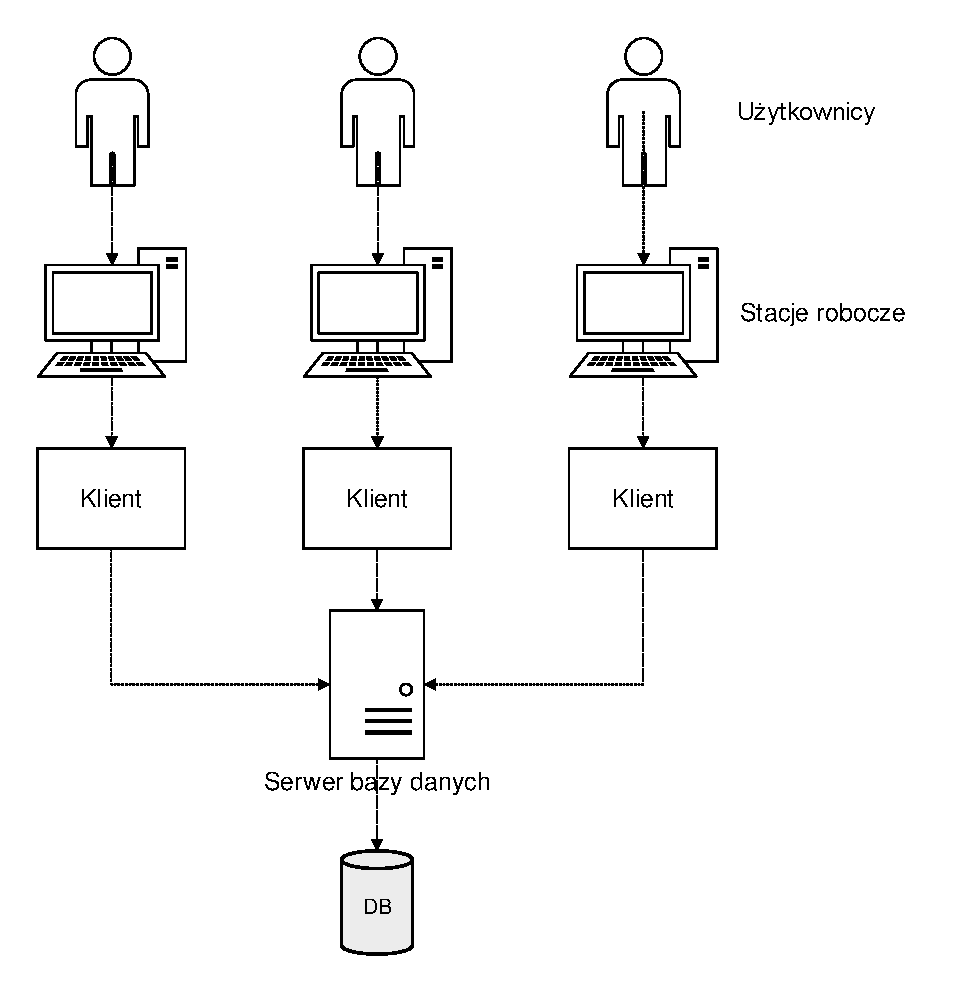
\includegraphics[width=10cm]{architecture-global.pdf}
	\caption{Schemat architektury systemu}
\end{figure}
Biorąc pod uwagę opisany powyżej charakter zamówionego rozwiązania, wybrana została prosta architektura z centralną bazą danych oraz aplikacją typu “gruby klient”, wykorzystującą bezpośrednie połączenie z bazą. Rozwiązanie to jest spójne z opisanymi cechami systemu, a poza tym jest dość proste we wdrożeniu i nie wprowadza niepotrzebnych kosztów rozproszenia.
\begin{figure}[H]
	\centering
	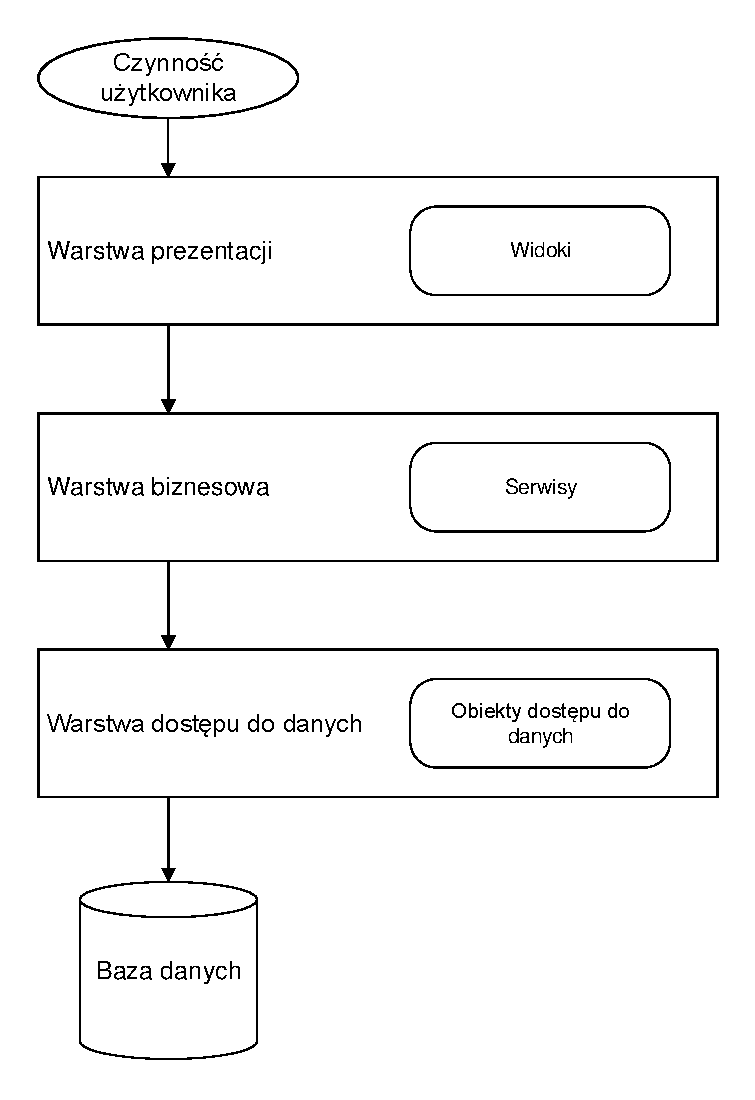
\includegraphics[width=8cm]{architecture-fat-client.pdf}
	\caption{Schemat architektury aplikacji klienckiej}
\end{figure}
Planowana architektura aplikacji klienckiej ma charakter warstwowy. Wyróżnione zostały następujące warstwy:
\begin{itemize}
	\item warstwa dostępu do danych - odpowiedzialna za kontakt z bazą oraz odczyt i zapis przechowywanych tam danych,
	\item warstwa biznesowa - odpowiedzialna za wykonywanie poszczególnych usług (np. dodania czy modyfikacji przewoźnika),
	\item warstwa prezentacji - odpowiedzialna za wyświetlanie interfejsu użytkownika.
	\end{itemize}
	Głównymi powodami zaproponowania architektury warstwowej były:
	\begin{itemize}
	\item możliwość wymiany silnika bazodanowego oraz warstwy prezentacji bez naruszania warstwy biznesowej,
	\item podział odpowiedzialności na poszczególne warstwy,
	\item spójny charakter wymagań - podział na podsystemy jest zbędny.
\end{itemize}
Ze względu na małą liczbę użytkowników niska skalowalność oraz wydajność rozwiązań warstwowych zostały uznane za ryzyko drugorzędne.

\section{Dokumentacja końcowa (powykonawcza)}

\subsection{Wymagania systemowe}
Aby zapewnić poprawne działanie systemu, wymagane są następujące komponenty:
\begin{enumerate}
	\item System operacyjny Windows 7 lub nowszy.
	\item MS SQL Server 2014 lub nowszy.
	\item .NET Framework 4.5.2 lub nowszy.
\end{enumerate}
% Punkt obowiązkowy.
%
% Rozdział powinien zawierać wymagania systemowe, wymagane oprogramowanie zewnętrzne
% (RDBMS, etc.)

\subsection{Biblioteki wraz z określeniem licencji}
% Punkt obowiązkowy.
%
% Rozdział powinien zawierać listę użytych bibliotek i komponentów firm trzecich wraz z ich licencjami.

\subsection{Instrukcja instalacji}
% Punkt obowiązkowy.
%
% Niniejszy rozdział powinien kompletną instrukcję instalacji systemu/aplikacji umożliwiająca osobie
% oceniającej implementację danego rozwiązania. Uwaga: instrukcja powinna być dostoswana do
% instalacji na czystym systemie operacyjnym.

\subsection{Instrukcja uruchomienia}
\begin{enumerate}
	\item W celu zapewnienia poprawnego uruchomienia aplikacji należy upewnić się, że instacja MS SQL serwera jest uruchomiona. Otwieramy \textbf{SQL Server Configuration Manager} i uruchamiamy instancję serwera (\textbf{MSSQLSERVER}), jeżeli jest wyłączona.
	\item Klikamy dwukrotnie plik wykonywalny \textbf{PublicTransport.exe}, aby uruchomić aplikację.
\end{enumerate}
% Punkt obowiązkowy.
% 
% Niniejszy rozdział powinien zawierać kompletną instrukcję uruchomienia systemu/aplikacji
% umożliwiającą osobie oceniającej weryfikację poprawności działania systemu.

\subsection{Instrukcja użycia}
% Punkt obowiązkowy.
%
% Niniejszy rozdział powinien zawierać kompletną instrukcję użycia (manual) systemu/aplikacji
% umożliwiająca osobie oceniającej weryfikację poprawności działania systemu.

\subsection{Instrukcja utrzymania}
Co kurwa...
% Punkt obowiązkowy.
%
% Niniejszy rozdział powinien zawierać kompletną instrukcję utrzymania systemu obejmującą procedury
% włączenia, wyłączenia systemu oraz procedury backup/restore.

\subsection{Raport odstępstw od specyfikacji wymagań}
% Punkt obowiązkowy.

\subsection{Dokumentacja usług Web Services}
% Punkt obowiązkowy
%
% Niniejszy rozdział powinien w przypadku, gdy system udostępnia publiczne usługi web services
% powinien zawierać dokumentację usług zamieszczone w formie opisowej lub np. wg specyfikacji
% swagger.

\section{Dokumentacja końcowa (powykonawcza) -- punkty wymagane przez prowadzącego zajęcia}

\subsection{Pseudokod}

\subsection{Diagramy sekwencji}
% Punkt obowiązkowy
%
% W przypadku projektów półsemestralnych lub dłuższych: w przypadku, gdy system składa się z
% komponentów rozproszonych należy dołączyć diagram(y) sekwencji. Rozdział zawierać powinien
% zawierać diagramy sekwencji opisujące komunikację pomiędzy systemami lub komponentami
% systemu. Należy w nim uwzględnić wszystkie przepływy komunikatów pomiędzy komponentami
% systemu lub systemami.

\subsection{Model danych}
Model danych użyty w systemie został przedstawiony w formie diagramu relacji na poniższej grafice:
\begin{center}
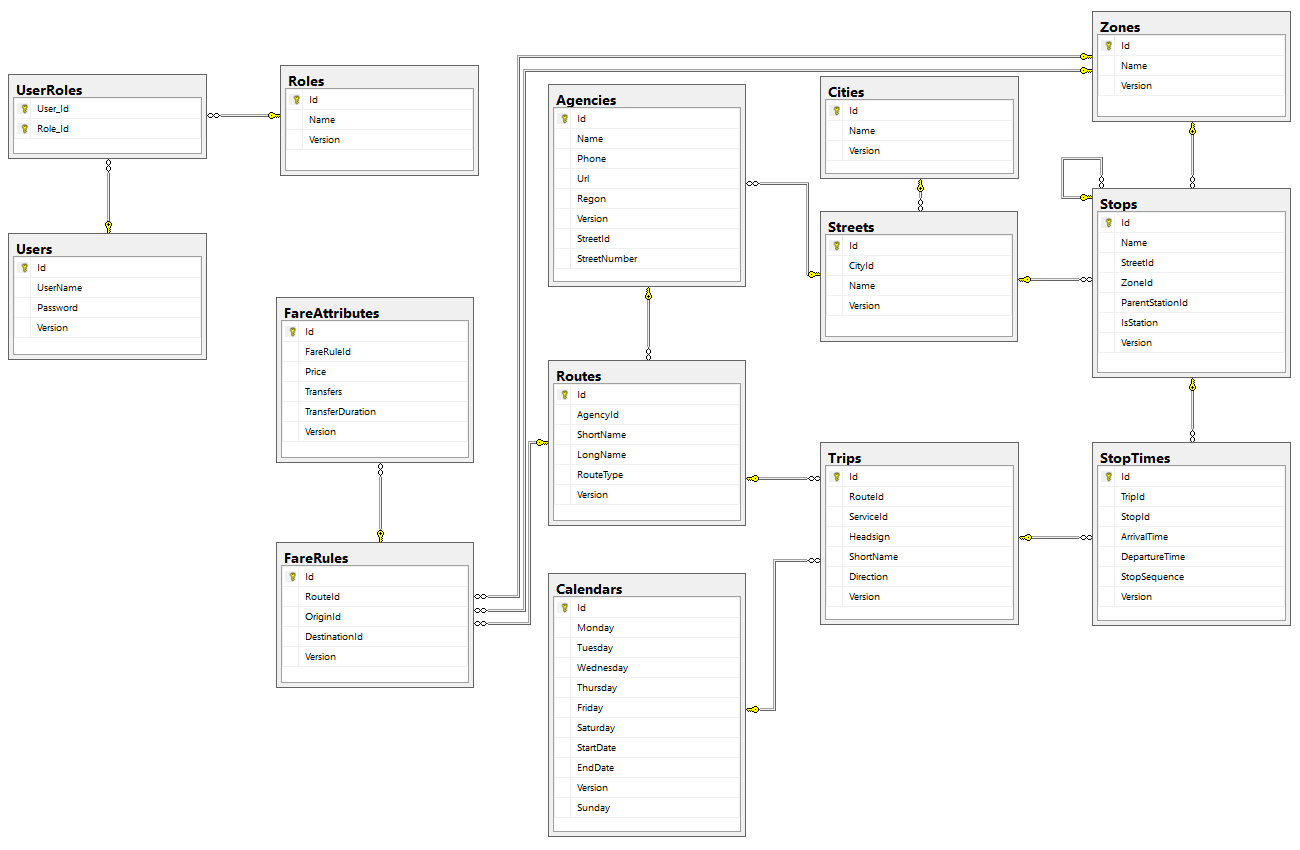
\includegraphics[scale = 0.33]{data-model.jpg}
\end{center}
Poniżej opisano znaczenie i rodzaj poszczególnych relacji zachodzących pomiędzy encjami w systemie.
\begin{enumerate}
	\item \textbf{User - Role} jest relacją wiele do wielu zrealizowaną przy pomocy tabeli pomocniczej UserRoles. Są to tabele niezależne od reszty systemu, ponieważ służą jedynie zdefiniowaniu elementów aplikacji dostępnych dla danego użytkownika.
	\item \textbf{City - Street} to relacja jeden do wielu. Ulice zdefiniowane w systemie zawierają informację o mieście, w którym są.
	\item Informacje o ulicy (a co za tym idzie również o mieście) zawarte są w poszczególnych agencjach (przewoźnikach) oraz przystankach, stąd relacje jeden do wielu \textbf{Street - Agency} oraz \textbf{Street - Stop}.
	\item Każdy przewoźnik zapewnia wiele połączeń różnymi środkami komunikacji, dlatego relacja \textbf{Agency - Route} jest relacją jeden do wielu.
	\item Poszczególne połączenia są jedynie definicją trasy. Sam przejazd (których może być wiele) pomiędzy punktami trasy zawarty jest w tabeli \textbf{Trips}. Przejazd musi zostać ponadto umieszczony w czasie, stąd dodatkowa tabela \textbf{Calendars}, która mówi w jakich dniach połączenie będzie funkcjonować. Tak określone relacje \textbf{Route - Trip} oraz \textbf{Calendar - Trip} są jeden do wielu.
	\item Należy również określić konkretne czasy postojów na trasie przejazdu. Tym zajmuje się tabela \textbf{StopTimes}, w której zdefiniowane poszczególne postoje są skojarzone z konkretnym przejazdem i przystankiem. To powoduje, że relacje \textbf{Trip - StopTime} oraz \textbf{Stop - StopTime} są jeden do wielu.
	\item Należy równiez zdefiniować strefy przejazdu, czym zajmuje się tabela \textbf{Zones}. Każdy przystanek ma przypisaną konkretną strefę w której się znajduje, więc relacja \textbf{Zone - Stop} jest jeden do wielu.
	\item TODO: Opis FareRule - FareAttribute oraz Route - FareAttribute
\end{enumerate}
% W przypadku projektów półsemestralnych lub dłuższych, gdy system składuje dane, należy opisać
% model danych. Model danych powinien być wyrażony przez diagram entity relationship w przypadku
% relacyjnej bazy danych. Zalecane jest wówczas opisanie znaczenia poszczególnych relacji, jak
% również czytelne oznaczenie rodzaju relacji (np. jeden do wielu) oraz kluczy głównych i kluczy obcych.
% W przypadku wykorzystania platform nierelacyjnych np. platform NoSQL lub składowania danych w
% plikach Apache Hadoop należy przedstawić opis konwencji zapisu danych. Jest to szczególnie istotne,
% gdy model danych jest prowadzony w trybie tzw. schema-on-read tzn. nie jest egzekwowany przez
% platformę składowania danych, a zależy wyłącznie od konwencji stosowanej przez aplikację np.
% konwencji nazewnictwa kolumn, treści wpisów w formacie JSON lub formatu sekwencji plików
% tworzonych w systemie plików HDFS.

\subsection{Scenariusz testów akceptacyjnych}
ROLA | CO TESTUJEMY | OPIS | CO WYJDZIE | WYSZŁO? | CO UMOŻLIWIA | UWAGI\\

Administrator\\
Dodanie nowego użytkownika\\
Wybranie zakładki Users na bocznym pasku aplikacji, przejście do widoku dodawania użytkownika po wciśnięciu przycisku Add New oraz zapisanie zmian przyciskiem Save.\\
Nowy użytkownik zostanie dodany do bazy danych.\\
Tak\\

Administrator\\
Modyfikacja istniejącego użytkownika\\
Wybranie zakładki Users na bocznym pasku aplikacji, wyszukanie istniejącego użytkownika, przejście do widoku edycji użytkownika po zaznaczeniu jednego z listy i wciśnięciu przycisku Edit Selected oraz zapisanie zmian przyciskiem Save.\\
Dane wybranego użytkownika zostaną zmodyfikowane.\\
Tak\\

Administrator\\
Usunięcie istniejącego użytkownika\\
Wybranie zakładki Users na bocznym pasku aplikacji, wyszukanie istniejącego użytkownika i wciśnięcie przycisku Delete Selected po wybraniu jednego z listy.\\
Dane wybranego użytkownika zostaną usunięte.\\
Tak\\

Użytkownik\\
Zalogowanie się\\
Wpisanie loginu i hasła w odpowiednie pola na ekranie logowania i wciśnięcie przycisku Login\\
Zalogowanie się do systemu w przypadku poprawnych danych, odmowa dostępu w przypadku niepoprawnych danych\\
Tak\\

Zalogowany użytkownik\\
Wylogowanie się\\
Wciśniecię przycisku Logout na bocznym pasku aplikacji.\\
Poprawne wylogowanie się z zystemu i przejście do ekranu logowania.\\
Tak\\

Pracownik\\
Dodanie nowego przewoźnika\\
Wybranie zakładki Agencies w bocznym pasku aplikacji, przejście do widoku dodania przewoźnika po wciśnięciu przycisku Add New oraz zapisanie zmian przyciskiem Save.\\
Nowy przewoźnik zostanie dodany do bazy danych.\\
Tak\\

Pracownik\\
Modyfiacja istniejącego przewoźnika\\
Wybranie zakładki Agencies na bocznym pasku aplikacji, wyszukanie istniejącego przewoźnika, przejście do widoku edycji przewoźnika po zaznaczeniu jednego z listy i wciśnięciu przycisku Edit Selected oraz zapisanie zmian przyciskiem Save.\\
Dane wybranego przewoźnika zostaną zmodyfikowane.\\
Tak\\

Pracownik\\
Usunięcie istniejącego przewoźnika\\
Wybranie zakładki Agencies na bocznym pasku aplikacji, wyszukanie istniejącego przewoźnika i wciśnięcie przycisku Delete Selected po wybraniu jednego z listy.\\
Dane wybranego przewoźnika zostaną usunięte.\\
Tak\\

Pracownik\\
Dodanie nowej linii połączeń\\
Wybranie zakładki Routes w bocznym pasku aplikacji, przejście do widoku dodania połączenia po wciśnięciu przycisku Add New oraz zapisanie zmian przyciskiem Save.\\
Nowe połączenie zostanie dodane do bazy danych.\\
Tak\\

Pracownik\\
Modyfikacja istniejącej linii połączeń\\
Wybranie zakładki Routes na bocznym pasku aplikacji, wyszukanie istniejącego połączenia, przejście do widoku edycji połączenia po zaznaczeniu jednego z listy i wciśnięciu przycisku Edit Selected oraz zapisanie zmian przyciskiem Save.\\
Dane dotyczące wybranego połączenia zostaną zmodyfikowane.\\
Tak\\

Pracownik\\
Usunięcie istniejącej linii połączeń\\
Wybranie zakładki Routes na bocznym pasku aplikacji, wyszukanie istniejącego połączenia i wciśnięcie przycisku Delete Selected po wybraniu jednego z listy.\\
Dane dotyczące wybranego połączenia zostaną usunięte.\\
Tak\\

Pracownik\\
Wyświetlanie połączeń przewoźnika\\
Wybranie zakładki Routes na bocznym pasku aplikacji i wybranie konkretnego przewoźnika w opcjach filtrowania.\\
Wyświetlona lista połączeń zapewnionych przez wybranego przewoźnika.\\
Tak\\

Pracownik\\
Wyświetlanie rozkładu jazdy\\
Wybranie zakładki Routes na bocznym pasku aplikacji, wyszukanie istniejącego połączenia i wciśnięcie przycisku Show Timetable po zaznaczeniu jednego z listy. Następnie przełączając się w liście przystanków po lewej możemy przeglądać godziny przyjazdu i odjazdu na ten przystanek dla danej linii.\\
Informacje o godzinach przyjazdu i odjazdu danej linii na konkretne przystanki.\\
Tak\\
% W przypadku projektów półsemestralnych np. realizowanych w ramach projektu zespołowego.
% Rozdział powinien zawierać scenariusze testów akceptacyjnych nawiązujących do wymagań
% funkcjonalnych i niefunkcjonalnych systemu.

\subsection{Raport z przeprowadzonych testów}
% W przypadku projektów półsemestralnych np. realizowanych w ramach projektu zespołowego.
% Rozdział powinien zawierać scenariusze testów akceptacyjnych nawiązujących do wymagań
% funkcjonalnych i niefunkcjonalnych systemu i wyniki ich przeprowadzenia.

\section{Lista użytych skrótów}

\renewcommand*{\refname}{\vspace*{-2em}}
\section{Bibliografia}
\begin{thebibliography}{99}
\end{thebibliography}
\end{document}
